\section{Aufbau}
\label{sec:Aufbau}
\begin{figure}
  \centering
  \begin{subfigure}{0.48\textwidth}
    \centering
    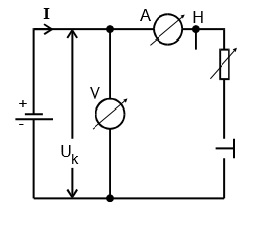
\includegraphics[height=5cm]{data/abb2.jpg}
    \caption{Messschschaltung zur Bestimmung von $U_0$ und $R_i$. \cite{V301}}
    \label{fig:abb2}
  \end{subfigure}
  \begin{subfigure}{0.48\textwidth}
    \centering
    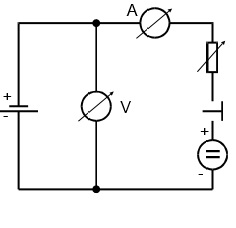
\includegraphics[height=5cm]{data/abb3.jpg}
    \caption{wie Abb.\ref{fig:abb2}, jedoch mit Verwendung einer Gegenspannung. \cite{V301}}
    \label{fig:abb3}
  \end{subfigure}
  \label{fig:Phasen}
\end{figure}
Es wird der Versuch entsprechend der Schaltbilder in Abb. \ref{fig:abb2} und Abb. \ref{fig:abb3} nacheinander aufgebaut.
Ein regelbarer Widerstand wird benutzt, in den für die Versuchsteile nötigen Ohm-Bereichen.